\section{METHODS}

\subsection{Digital Phantom}
Based on the fiber geometries of the digital phantom 
created for the High angular resolution diffusion imaging 
reconstruction Challenge held in ISBI 2013 
(San Francisco, US), we simulated high resolution 
(0.5mm isotropic) T1 (TE/TR=10/1500ms) and T2 
(TE/TR=90/5000ms) images, as well as a \gls*{dmri}
(1.0mm isotropic, $b$=1200, 32 evenly-distributed 
directions, 1 B0 image) image.
The phantom includes \gls*{wm} fiber bundles, 
\gls*{csf} and \gls*{gm}. Diffusion is modeled by a 
restricted and a hindered compartment, similar to
\cite{assaf_composite_2005}.

\subsection{Theory-based synthetic distortion}

Fieldmap-based correction methodologies
\cite{jezzard_correction_1995} use a map
of the field in the scanner. More precisely, the
phase difference between two subsequent samplings
of the fieldmap. With that information, it is possible
to compute the theoretical displacement that each
voxel is to suffer, the so-called \gls*{vsm}. The
most prominent feature of this \gls*{vsm} is that all
the shifts have the same orientation (parallel to the
phase-encoding direction of the \gls*{epi}) and their
magnitude and direction depend on the \gls*{epi} 
gradient increments (or \emph{blips}), and the actual
phase difference at the voxel.

In order to create a realistic distortion, we
generated a synthetic phase-difference map 
consistent with the phantom.  We defined two regions 
of smooth de-phasing (up to $0.05\pi$ rad. excursions) 
and computed the corresponding \gls*{vsm}, using the 
tools distributed with the \texttt{FSL} package 
\cite{jenkinson_fsl_2012}  and
standard parameters ($\Delta$TE=2.46ms for the
fieldmap and \emph{effective dwell time} of 
0.77ms for the \gls*{epi}).

Once a realistic \gls*{vsm} was available, we generated
the corresponding distorted \glspl*{dwi}, in two opposed
phase-gradient encoding directions. The second simulated
``acquisition'' of the same phantom was necessary 
for evaluating the second family of correction methods.

In this simple manner, we generated a full gold-standard
protocol, containing realistic T1 and T2
at high resolution, \glspl*{dwi} acquired in two
different phase encoding directions, and a ground-truth
\gls*{dwi} data, which is not available for real datasets.


\begin{figure}[thpb]
   \centering
   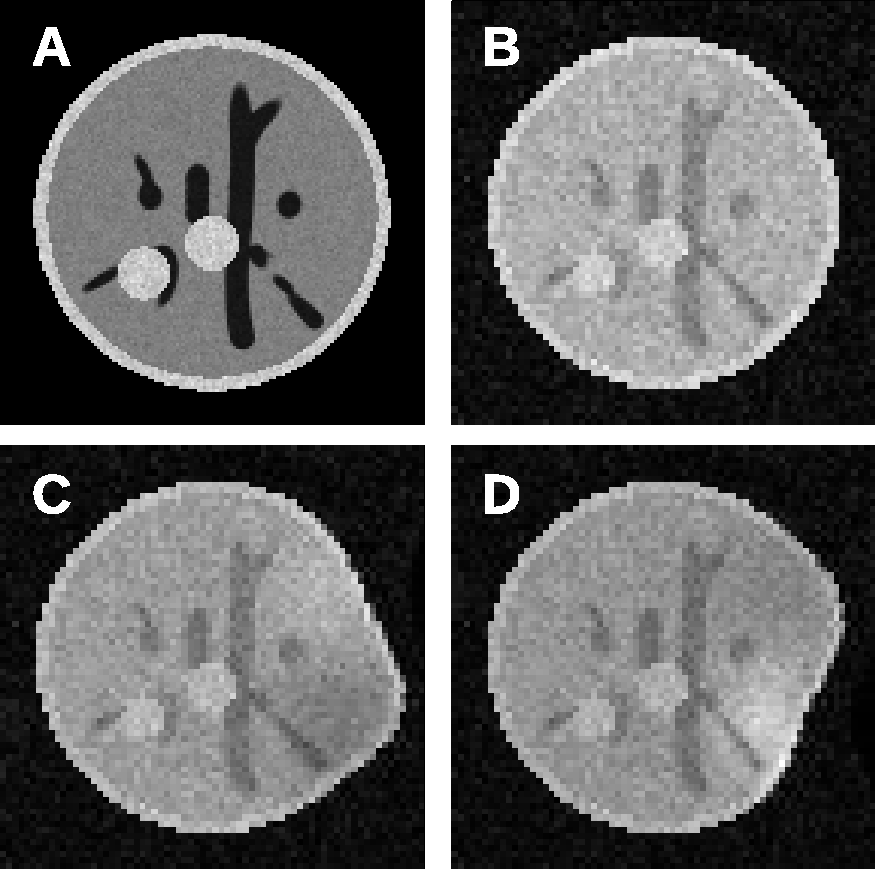
\includegraphics[width=0.8\columnwidth]{Fig01-Phantom}
   \caption{Original and distorted digital phantom (sagittal
   planes). A) T2-weighted image; B) undistorted B0 volume;
   C and D) distorted B0 volumes with opposed phase encoding 
   directions.}
   \label{fig:label}
\end{figure}

\subsection{Correction methods}

\paragraph*{\Gls*{fmb}} As it was previously described,
this family of correction technologies infer a \gls*{vsm}
from the phase difference map. In this work, we use the
tool \texttt{fugue} \cite{jenkinson_fsl_2012} aforementioned.

\paragraph*{\Gls*{reb}} We use the tool
\texttt{topup} from \cite{jenkinson_fsl_2012} to correct
using the B0 of a reverse-encoding simulation of the \gls*{dti}.
In this second case, the \gls*{vsm} is inferred from the
differences between the two corresponding B0. This technique
also uses least-squares-fitting to interpolate the undistorted
signal, and therefore provides with a robust dropout correction.

\paragraph*{\Gls*{t2b}} For this last methodology
we fine-tuned the \texttt{ANTs} tool \cite{avants_ants:_2013},
in order that registering the B0 to the T2. Additionally,
undistorted images are corrected for dropout using the determinant
of the Jacobian of the deformation field.

\subsection{Evaluation}

\paragraph*{Proposed workflows}
We used \texttt{nipype} \cite{gorgolewski_nipype:_2011}
to conveniently integrate the correction methods in
comprehensive evaluation workflows:

\begin{itemize}
\item \textbf{Phantom deformation}: We release the pipeline
that generates the gold-standard, along with
distorted versions of the \glspl*{tpm} for
evaluation purposes.
\item \textbf{Correction workflow}: A high-level pipeline
integrates the three proposed correction methods,
ensuring that all the requirements for inputs are
met. As outputs this workflow produces the different
corrected versions of the phantom (\gls*{fmb}, \gls*{reb}
and \gls*{t2b}) alongside corrected versions of the
distorted \glspl*{tpm}.
\item \textbf{Reconstruction workflow}: This pipeline uses
the Diffusion Toolkit \cite{wang_diffusion_2007}, 
to produce deterministic tractography
from \gls*{dmri} data at the input. Therefore,
tractographies of original, and recovered data
are produced for comparison.
\item \textbf{Benchmarking workflow}: The final processing
element collects all the outputs from the previous
workflows and extracts the evaluation scores.
\end{itemize}
General-purpose 
workflows have been contributed to the upstream code
of the tool, under the branch \texttt{nipype.workflows.dmri}.
Testing-specific workflows are also publicly released.

\paragraph*{Evaluation scores}
We evaluated three characteristics of the corrected
phantom. First, we assessed the geometrical correctness
and reported overlap indices of three \glspl*{tpm} 
(namely \gls*{csf},\gls*{wm}, and \gls*{gm}).
More precisely, we computed the \gls*{fji} as 
proposed in \cite{crum_generalized_2006} weighted by 
the volumes of labels. 
Second, to evaluate the quality of the actual 
signal \emph{sanity} after recovery (dropout 
correction), we studied the signal similarity
frame by frame computing the $\ell_1$-norm
based correlation index. We report this score
on the B0 and the average of the remaining 32 
\glspl*{dwi}. Third, we report the 
impact on tractography using the \gls*{frr}, that 
informs the number of recovered fibers versus the 
gold-standard number for a specific reconstruction
method.
